\documentclass{article}
\usepackage{graphicx}
\usepackage{amsmath}
\usepackage{amssymb}
\usepackage{enumitem}
\usepackage{listings}
\usepackage[margin=1in]{geometry}
\usepackage{xcolor}
\usepackage{tikz}
\usetikzlibrary{shapes, arrows, positioning, calc}
\usepackage{tcolorbox}

% Define colors for syntax highlighting
\definecolor{codegreen}{rgb}{0,0.6,0}
\definecolor{codegray}{rgb}{0.5,0.5,0.5}
\definecolor{codepurple}{rgb}{0.58,0,0.82}
\definecolor{backcolour}{rgb}{0.95,0.95,0.92}

% Python style for highlighting
\lstdefinestyle{pythonstyle}{
   backgroundcolor=\color{backcolour},  
   commentstyle=\color{codegreen},
   keywordstyle=\color{magenta},
   numberstyle=\tiny\color{codegray},
   stringstyle=\color{codepurple},
   basicstyle=\ttfamily\footnotesize,
   breakatwhitespace=false,     
   breaklines=true,          
   captionpos=b,            
   keepspaces=true,          
   numbers=left,            
   numbersep=5pt,          
   showspaces=false,          
   showstringspaces=false,
   showtabs=false,          
   tabsize=2
}
\lstset{style=pythonstyle}

\title{Lecture: Self-Attention and the Transformer Revolution\\
From Sequential Processing to Parallel Computation}
\author{Deep Learning Class}
\date{\today}

\begin{document}
\maketitle


Last lecture, we solved the seq2seq bottleneck problem using \textbf{cross-attention}. We built an attention-augmented RNN where:

\begin{itemize}
\item The \textbf{encoder RNN} processes the source sequence to build a memory bank $\{h_1, h_2, \ldots, h_T\}$
\item The \textbf{decoder RNN} generates the target sequence step-by-step
\item At each decoding step $t$, \textbf{cross-attention} lets the decoder query the encoder memory to compute a dynamic context vector $c_t$
\end{itemize}

This solved the information bottleneck. Translation quality improved dramatically. Models could handle longer sequences. The approach was state-of-the-art from 2015--2017.

But we still have a fundamental problem.

\section{The Remaining challenge: RNNs are inherently sequential}
\textbf{RNNs are inherently sequential}. At each time step $t$:
\[
h_t = f(h_{t-1}, x_t)
\]

You \textbf{cannot} compute $h_t$ until you have computed $h_{t-1}$. This means:

\begin{itemize}
\item \textbf{No parallelization} during the forward pass
\item \textbf{Long training times} for sequences with hundreds or thousands of tokens
\item \textbf{GPU underutilization}: Your expensive GPU sits mostly idle, waiting for the sequential computation to complete
\end{itemize}

Compare this to CNNs, which we know are highly parallel. For example translating a sentence with 100 source tokens and 80 target tokens via RNN:

\begin{itemize}
\item \textbf{Encoder}: Must process 100 tokens sequentially $\rightarrow$ 100 serial steps
\item \textbf{Decoder}: Must generate 80 tokens sequentially $\rightarrow$ 80 serial steps
\item \textbf{Total}: At least 180 sequential operations per training example
\end{itemize}

With a batch size of 32, you still need 180 sequential steps, and only 32 examples run in parallel. Your GPU with thousands of cores is vastly underutilized.

For a dataset with 10 million sentence pairs, training takes weeks on multiple GPUs.

\subsection{Beyond Training: Encoding Long-Range Dependencies}

Even with LSTMs and GRUs, capturing dependencies across 100+ time steps remains difficult:

\begin{itemize}
\item Gradients must backpropagate through many time steps
\item Information gets compressed at each step (despite gating)
\item The first token's representation has been transformed 100+ times before reaching the final output
\end{itemize}

Last lecture, we learned that attention can dynamically access information without compression.

Could we use attention to \textbf{replace} recurrence entirely, instead of just augmenting it?

If we could, we would get:
\begin{itemize}
\item \textbf{Parallel computation} (like CNNs)
\item \textbf{Flexible long-range dependencies} (like attention)
\item \textbf{No sequential bottleneck} (unlike RNNs)
\end{itemize}


\subsubsection{The Search for Parallelism: Why Not CNNs?}

If we want parallelism, why not use Convolutional Neural Networks (CNNs)? They are highly parallelizable and work well for images.

CNNs excel with images because nearby pixels are highly correlated (strong local correlation). Text is different. The most critical relationships can span long distances.

\begin{center}
   \textit{``The \textbf{dog} chased its own \textbf{tail}.''}
\end{center}

A standard CNN struggles to connect ``dog" and ``tail" efficiently. Information must pass through many layers, degrading the signal.

% CNN limitation diagram
\begin{center}
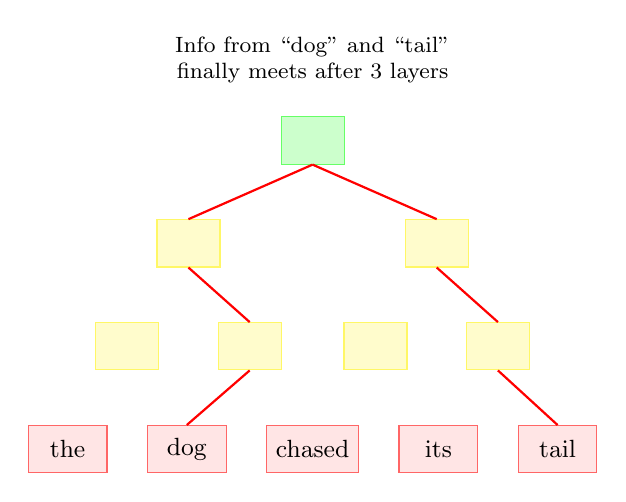
\begin{tikzpicture}[
   word/.style={rectangle, draw=red!60, fill=red!10, minimum width=1cm, minimum height=0.6cm, font=\small},
   c1/.style={rectangle, draw=yellow!60, fill=yellow!20, minimum width=0.8cm, minimum height=0.6cm},
   c2/.style={rectangle, draw=green!60, fill=green!20, minimum width=0.8cm, minimum height=0.6cm},
   highlight/.style={red, thick, rounded corners},
   node distance=0.3cm and 0.5cm
]
   % Words
   \node[word] (w1) {the};
   \node[word, right=of w1] (w2) {dog};
   \node[word, right=of w2] (w3) {chased};
   \node[word, right=of w3] (w4) {its};
   \node[word, right=of w4] (w5) {tail};
  
   % Layer 1
   \node[c1, above=1cm of $(w1)!0.5!(w2)$] (l1_1) {};
   \node[c1, above=1cm of $(w2)!0.5!(w3)$] (l1_2) {};
   \node[c1, above=1cm of $(w3)!0.5!(w4)$] (l1_3) {};
   \node[c1, above=1cm of $(w4)!0.5!(w5)$] (l1_4) {};
  
   % Layer 2
   \node[c1, above=1cm of $(l1_1)!0.5!(l1_2)$] (l2_1) {};
   \node[c1, above=1cm of $(l1_3)!0.5!(l1_4)$] (l2_2) {};
  
   % Layer 3 (top)
   \node[c2, above=1cm of $(l2_1)!0.5!(l2_2)$] (l3_1) {};
  
   % Highlight paths from dog and tail
   \draw[highlight] (w2.north) -- (l1_2.south);
   \draw[highlight] (l1_2.north) -- (l2_1.south);
   \draw[highlight] (l2_1.north) -- (l3_1.south);
  
   \draw[highlight] (w5.north) -- (l1_4.south);
   \draw[highlight] (l1_4.north) -- (l2_2.south);
   \draw[highlight] (l2_2.north) -- (l3_1.south);
  
   % Annotation
   \node[above=0.3cm of l3_1, text width=4cm, align=center, font=\footnotesize] {Info from ``dog'' and ``tail'' finally meets after 3 layers};
\end{tikzpicture}
\end{center}



\section{The Radical Idea: Self-Attention}

\subsection{Attention Doesn't Care Where Q, K, V Come From}

Recall the general attention formula from last lecture:

\[
\text{Attention}(Q, K, V) = \text{softmax}\left(\frac{QK^T}{\sqrt{d_k}}\right)V
\]

\begin{itemize}
\item $Q$ (queries): ``What am I looking for?''
\item $K$ (keys): ``What do I offer?''
\item $V$ (values): ``What content do I provide?''
\end{itemize}

In \textbf{cross-attention} (last lecture):
\begin{itemize}
\item $Q$ comes from the \textit{decoder} (the query side)
\item $K, V$ come from the \textit{encoder} (the memory bank)
\item Attention connects two \textit{different} sequences
\end{itemize}

But mathematically, there's no requirement that $Q$, $K$, and $V$ come from different places!

\subsection{What if Q, K, V All Come From the Same Sequence?}

\begin{tcolorbox}[colback=green!5!white, colframe=green!50!black, title=Self-Attention: The Core Idea]
\textbf{Self-Attention} is when the queries, keys, and values all come from the \textit{same} sequence.

Given an input sequence $X = [x_1, x_2, \ldots, x_n] \in \mathbb{R}^{n \times d}$:

\begin{align}
Q &= XW_Q \quad \text{(query: ``What am I looking for in my neighbors?'')}\\
K &= XW_K \quad \text{(key: ``What do I offer to others?'')}\\
V &= XW_V \quad \text{(value: ``What information do I contain?'')}
\end{align}

Each position in the sequence can attend to \textit{every other position} (including itself) to gather context.
\end{tcolorbox}

\subsection{A Linguistic Analogy: Understanding ``Bank''}

Consider the sentence:
\begin{center}
\textit{``The bank by the river offers great views of the boats.''}
\end{center}

To understand what ``bank'' means in this context:
\begin{itemize}
\item The word ``bank'' (at position 2) acts as a \textbf{query}: ``What are my neighbors telling me about my meaning?''
\item It looks at ``river'' (key: ``I'm related to water''), ``offers'' (key: ``I might be a financial institution''), ``boats'' (key: ``I'm related to water'')
\item The model computes attention weights: high attention to ``river'' and ``boats'', low attention to ``offers''
\item It combines the representations (values) from these neighbors to disambiguate: this is a \textit{riverbank}, not a financial bank
\end{itemize}

\textbf{Crucially}: This all happens \textit{within} the sentence itself. Each word refines its representation by attending to related words.

\begin{center}
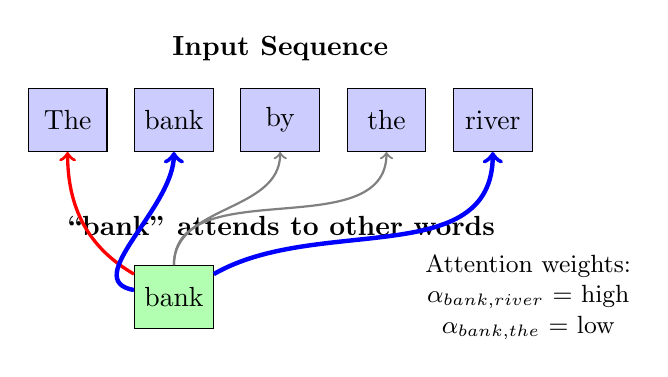
\begin{tikzpicture}[scale=0.9]
% Input sequence
\node[align=center] at (3, 4) {\textbf{Input Sequence}};
\foreach \x/\word in {0/The, 1/bank, 2/by, 3/the, 4/river} {
   \node[draw, rectangle, minimum width=1cm, minimum height=0.8cm, fill=blue!20] (w\x) at (\x*1.5, 3) {\word};
}

% Attention from ``bank"
\node[align=center] at (3, 1.5) {\textbf{``bank'' attends to other words}};
\node[draw, rectangle, minimum width=1cm, minimum height=0.8cm, fill=green!30] (query) at (1.5, 0.5) {bank};

% Attention weights (thicker = higher weight)
\draw[->, very thick, red] (query) to[out=150, in=270] (w0);
\draw[->, ultra thick, blue] (query) to[out=170, in=270] (w1);
\draw[->, thick, gray] (query) to[out=90, in=270] (w2);
\draw[->, thick, gray] (query) to[out=90, in=270] (w3);
\draw[->, ultra thick, blue] (query) to[out=30, in=270] (w4);

\node[align=center, font=\small] at (6.5, 0.5) {Attention weights:\\$\alpha_{bank, river}$ = high\\$\alpha_{bank, the}$ = low};
\end{tikzpicture}
\end{center}

Each word simultaneously:
\begin{itemize}
\item Acts as a \textbf{query} (attends to others)
\item Acts as a \textbf{key} (is attended to by others)
\item Provides a \textbf{value} (contributes its representation)
\end{itemize}


\subsubsection{The Autoregressive Property \& Causal Masking in the Decoder}

During training, we know the entire target sequence. But during inference, we generate one token at a time.

\begin{tcolorbox}[colback=red!5!white, colframe=red!75!black, title=The Cheating Problem]
Without masking, the decoder's self-attention at position $t$ could attend to position $t+1, t+2, \ldots$ (future tokens).

This is \textbf{cheating}! During inference, those future tokens don't exist yet.

The model would learn to ``peek at the answer'' during training, then fail completely at test time.
\end{tcolorbox}



In the decoder's self-attention, we apply a \textbf{causal mask} (also called an autoregressive mask):

\begin{center}
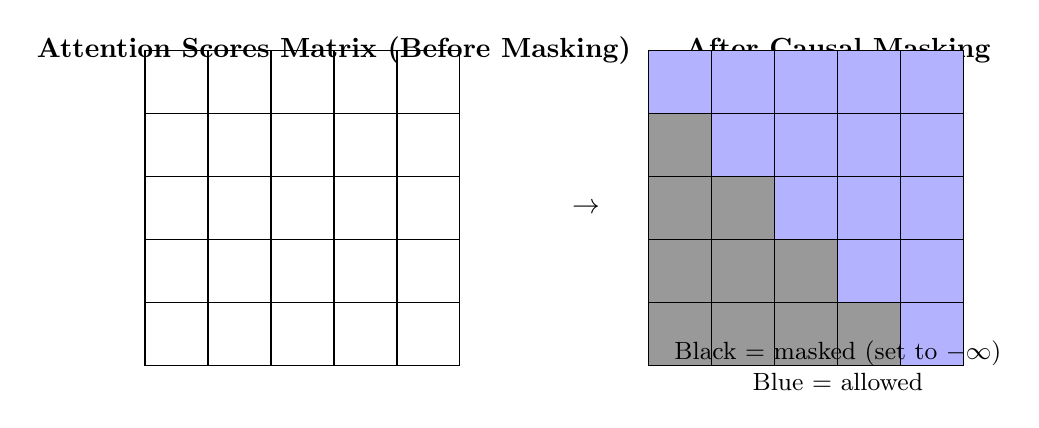
\begin{tikzpicture}[scale=0.8]
\node[align=center] at (3, 4) {\textbf{Attention Scores Matrix (Before Masking)}};

% Draw matrix
\foreach \x in {0,1,2,3,4} {
   \foreach \y in {0,1,2,3,4} {
     \draw (\x, 3-\y) rectangle (\x+1, 4-\y);
   }
}

\node[align=center] at (7, 1.5) {$\rightarrow$};

\node[align=center] at (11, 4) {\textbf{After Causal Masking}};

% Draw masked matrix
\foreach \x in {0,1,2,3,4} {
   \foreach \y in {0,1,2,3,4} {
     \pgfmathsetmacro{\fill}{ifthenelse(\y>\x,"black!40","blue!30")}
     \draw[fill=\fill] (\x+8, 3-\y) rectangle (\x+9, 4-\y);
   }
}

\node[align=center, font=\small] at (11, -1) {Black = masked (set to $-\infty$)\\Blue = allowed};
\end{tikzpicture}
\end{center}

Position $i$ can only attend to positions $j \leq i$ (itself and previous positions).

% \textbf{Implementation}:
% \begin{lstlisting}[language=Python, caption=Causal Mask]
% def create_causal_mask(seq_len):
%    # Create upper triangular matrix of -inf
%    mask = torch.triu(torch.ones(seq_len, seq_len) * float('-inf'), 
%              diagonal=1)
%    return mask  # Shape: (seq_len, seq_len)

% # In attention computation:
% scores = torch.matmul(Q, K.transpose(-2, -1)) / math.sqrt(d_k)
% scores = scores + causal_mask  # Add -inf to future positions
% attention_weights = torch.softmax(scores, dim=-1)
% \end{lstlisting}



\section{The Mathematics of Self-Attention}

\subsection{Step-by-Step Computation}

Given an input sequence $X \in \mathbb{R}^{n \times d_{model}}$ where:
\begin{itemize}
\item $n$ is the sequence length
\item $d_{model}$ is the embedding dimension
\end{itemize}

\textbf{Step 1: Project to Q, K, V spaces}
\begin{align}
Q &= XW_Q \in \mathbb{R}^{n \times d_k}\\
K &= XW_K \in \mathbb{R}^{n \times d_k}\\
V &= XW_V \in \mathbb{R}^{n \times d_v}
\end{align}

where $W_Q, W_K \in \mathbb{R}^{d_{model} \times d_k}$ and $W_V \in \mathbb{R}^{d_{model} \times d_v}$ are learnable projection matrices.

\textbf{Step 2: Compute attention scores}
\[
\text{Scores} = \frac{QK^T}{\sqrt{d_k}} \in \mathbb{R}^{n \times n}
\]

The $(i,j)$ entry measures how much position $i$ should attend to position $j$.

\textbf{Step 3: Apply softmax to get attention weights}
\[
\text{Attention Weights} = \text{softmax}(\text{Scores}) \in \mathbb{R}^{n \times n}
\]

Each row sums to 1, giving a probability distribution over positions to attend to.

\textbf{Step 4: Weighted combination of values}
\[
\text{Output} = \text{Attention Weights} \cdot V \in \mathbb{R}^{n \times d_v}
\]

Putting It All Together:

\[
\text{SelfAttention}(X) = \text{softmax}\left(\frac{(XW_Q)(XW_K)^T}{\sqrt{d_k}}\right)(XW_V)
\]

\textbf{Key properties:}
\begin{enumerate}
\item \textbf{Permutation equivariant}: If you shuffle the input, the output shuffles in the same way
\item \textbf{Parallel computation}: All positions can compute their attention simultaneously
\item \textbf{All-to-all connections}: Every position can directly attend to every other position in one step
\item \textbf{No parameters depend on sequence length}: The same $W_Q, W_K, W_V$ work for any $n$
\end{enumerate}

\section{The Critical Problem: Where Did the Sequence Order Go?}

\subsection{Self-Attention is a Bag of Vectors}

Consider the attention output for position $i$:
\[
\text{output}_i = \sum_{j=1}^{n} \alpha_{ij} v_j
\]

This is a \textbf{weighted sum}. Weighted sums are \textbf{permutation invariant}!

\begin{tcolorbox}[colback=red!5!white, colframe=red!75!black, title=The Bag of Vectors Problem]
If we shuffle the input sequence, the self-attention output at each position remains exactly the same (after unshuffling).

Self-attention has \textbf{no notion of order}!

For the sentences:
\begin{itemize}
\item ``The cat chased the mouse''
\item ``The mouse chased the cat''
\end{itemize}

Self-attention would produce identical representations (up to position shuffling). But these sentences have \textbf{opposite meanings}!
\end{tcolorbox}

\subsection{Why This Wasn't a Problem Before}

In our attention-augmented RNN:
\begin{itemize}
\item The \textbf{RNN} encodes positional information through its recurrent connections
\item Hidden state $h_t$ inherently depends on $h_{t-1}$, which depends on $h_{t-2}$, etc.
\item The RNN provides the sequential inductive bias
\item Attention just \textit{augments} this with dynamic access
\end{itemize}

But if we \textit{remove} the RNN and use \textit{only} self-attention, we lose all positional information!

\section{The Solution: Positional Encoding}
Since self-attention has no notion of order, we must \textbf{explicitly} provide positional information.

\begin{tcolorbox}[colback=green!5!white, colframe=green!50!black, title=Positional Encoding Strategy]
\textbf{Before} feeding embeddings into the self-attention layer, we add a position-dependent signal:

\[
\text{Input to Self-Attention} = \text{Token Embedding} + \text{Positional Encoding}
\]

The positional encoding is a vector that encodes the position in the sequence.
\end{tcolorbox}

\subsection{Desiderata for Positional Encodings}

What properties should our positional encoding have?

\begin{enumerate}
\item \textbf{Unique}: Each position should get a different encoding
\item \textbf{Bounded}: Values shouldn't grow without bound (for numerical stability)
\item \textbf{Deterministic}: Same position should always get the same encoding
\item \textbf{Generalizable}: Should work for sequences longer than those seen during training
\item \textbf{Relative information}: Ideally, the model can learn about relative positions (e.g., ``word 3 positions to the left'')
\end{enumerate}

% \subsection{The Sinusoidal Positional Encoding}

% The Transformer paper (Vaswani et al., 2017) proposed using sine and cosine functions:

% \begin{align}
% PE_{(pos, 2i)} &= \sin\left(\frac{pos}{10000^{2i/d_{model}}}\right)\\
% PE_{(pos, 2i+1)} &= \cos\left(\frac{pos}{10000^{2i/d_{model}}}\right)
% \end{align}

% where:
% \begin{itemize}
% \item $pos$ is the position in the sequence (0, 1, 2, \ldots)
% \item $i$ is the dimension index (0, 1, \ldots, $d_{model}/2 - 1$)
% \item Even dimensions use sine, odd dimensions use cosine
% \end{itemize}

% \subsection{Why Sine and Cosine?}

% \textbf{Intuition 1: Different Frequencies}

% Each dimension uses a different frequency:
% \begin{itemize}
% \item Low dimensions (small $i$): High frequency $\rightarrow$ changes rapidly with position
% \item High dimensions (large $i$): Low frequency $\rightarrow$ changes slowly with position
% \end{itemize}

% This is like the binary representation idea: different ``bits'' encode position at different granularities.

% \textbf{Intuition 2: Relative Position via Linear Transformation}

% For any fixed offset $\phi$, we can express $PE_{pos+\phi}$ as a \textit{linear function} of $PE_{pos}$:

% \[
% \begin{bmatrix}
% \cos(\omega \phi) & \sin(\omega \phi) \\
% -\sin(\omega \phi) & \cos(\omega \phi)
% \end{bmatrix}
% \begin{bmatrix}
% \sin(\omega \cdot pos) \\
% \cos(\omega \cdot pos)
% \end{bmatrix}
% =
% \begin{bmatrix}
% \sin(\omega \cdot (pos + \phi)) \\
% \cos(\omega \cdot (pos + \phi))
% \end{bmatrix}
% \]

% This means the model can learn to attend to relative positions (``3 words ago'') via learned linear transformations.

% \textbf{Intuition 3: Bounded and Smooth}

% \begin{itemize}
% \item Sine and cosine are bounded: $[-1, 1]$
% \item They are smooth and continuous (helpful for interpolation to unseen positions)
% \item They are periodic but with very long periods for higher dimensions
% \end{itemize}

% \subsection{Visualizing Positional Encodings}

% \begin{center}
% \begin{tikzpicture}[scale=0.7]
% \draw[->] (0,0) -- (10,0) node[right] {Position};
% \draw[->] (0,0) -- (0,6) node[above] {Encoding Dimension};

% % Simulate heatmap with rectangles
% \foreach \x in {0,0.5,...,9.5} {
%    \foreach \y in {0,0.3,...,5.7} {
%     \pgfmathsetmacro{\val}{sin((\x*20 + \y*50))}
%     \pgfmathsetmacro{\col}{(\val + 1) * 50}
%     \fill[blue!\col!white] (\x, \y) rectangle (\x+0.5, \y+0.3);
%    }
% }

% \node[align=center, font=\small] at (5, -1) {Lower dimensions: high frequency\\Higher dimensions: low frequency};
% \end{tikzpicture}
% \end{center}

% Each row is a dimension, each column is a position. The pattern shows how different dimensions encode position at different frequencies.

\section{Comparing Architectures: CNNs, RNNs, and Self-Attention}

Now we can understand the trade-offs between architectures:

\begin{center}
\begin{tabular}{|l|c|c|c|}
\hline
\textbf{Property} & \textbf{CNN} & \textbf{RNN} & \textbf{Self-Attention} \\
\hline
Parallel Computation & \checkmark & $\times$ & \checkmark \\
\hline
Max Path Length & $O(\log n)$ & $O(n)$ & $O(1)$ \\
\hline
Computational Complexity & $O(n \cdot k \cdot d^2)$ & $O(n \cdot d^2)$ & $O(n^2 \cdot d)$ \\
\hline
Sequential Operations & $O(1)$ & $O(n)$ & $O(1)$ \\
\hline
Positional Encoding & Implicit (local) & Implicit (recurrence) & Explicit (added) \\
\hline
Long-Range Dependencies & Difficult & Medium & Easy \\
\hline
Best For & Local patterns & Sequential data & Global context \\
\hline
\end{tabular}
\end{center}

\subsection{Understanding the Complexity}

\textbf{RNN}: $O(n \cdot d^2)$
\begin{itemize}
\item $n$ sequential steps, each involves $d \times d$ matrix multiplication
\item \textbf{Cannot parallelize} across the sequence
\end{itemize}

\textbf{Self-Attention}: $O(n^2 \cdot d)$
\begin{itemize}
\item Computing $QK^T$: $(n \times d) \times (d \times n) = n^2 \cdot d$ operations
\item \textbf{Fully parallelizable} across all positions
\item \textbf{Trade-off}: Quadratic in sequence length, but parallelizable
\end{itemize}

\textbf{The Key Insight}: For sequences up to a few thousand tokens, $O(n^2 \cdot d)$ with parallelization is faster than $O(n \cdot d^2)$ without parallelization on modern hardware.

\subsection{Maximum Path Length}

The \textbf{maximum path length} is the longest path between any two positions in the network.

\begin{itemize}
\item \textbf{RNN}: $O(n)$ -- information from position 1 must pass through positions 2, 3, \ldots, $n-1$ to reach position $n$
\item \textbf{CNN}: $O(\log n)$ with deep stacks -- information flows hierarchically
\item \textbf{Self-Attention}: $O(1)$ -- every position can directly attend to every other position in a single step
\end{itemize}

Shorter paths mean:
\begin{itemize}
\item Easier gradient flow during backpropagation
\item More direct modeling of long-range dependencies
\item Less information compression
\end{itemize}

\section{The Transformer Architecture: Putting It All Together}

\subsection{High-Level Overview}

The Transformer replaces RNNs with a stack of self-attention layers:

\begin{center}
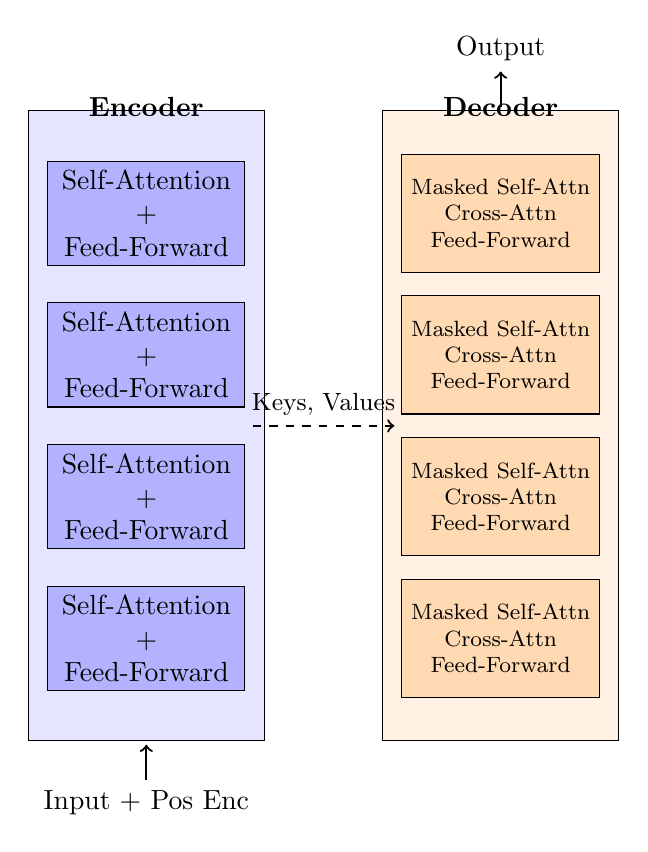
\begin{tikzpicture}[scale=0.9]
% Encoder stack
\node[draw, rectangle, minimum width=3cm, minimum height=8cm, fill=blue!10] (enc) at (0,0) {};
\node[align=center] at (0, 4.5) {\textbf{Encoder}};

\foreach \y in {-3,-1,1,3} {
   \node[draw, rectangle, minimum width=2.5cm, minimum height=1.2cm, fill=blue!30, align=center] at (0, \y) {Self-Attention\\+\\Feed-Forward};
}

% Decoder stack
\node[draw, rectangle, minimum width=3cm, minimum height=8cm, fill=orange!10] (dec) at (5,0) {};
\node[align=center] at (5, 4.5) {\textbf{Decoder}};

\foreach \y in {-3,-1,1,3} {
   \node[draw, rectangle, minimum width=2.5cm, minimum height=1.5cm, fill=orange!30, align=center, font=\footnotesize] at (5, \y) {Masked Self-Attn\\Cross-Attn\\Feed-Forward};
}

% Input/Output
\draw[<-, thick] (0, -4.5) -- (0, -5) node[below] {Input + Pos Enc};
\draw[->, thick] (5, 4.5) -- (5, 5) node[above] {Output};

% Connection between encoder and decoder
\draw[->, thick, dashed] (1.5, 0) -- (3.5, 0) node[midway, above, font=\small] {Keys, Values};
\end{tikzpicture}
\end{center}

\textbf{Key components:}
\begin{enumerate}
\item \textbf{Input Embeddings + Positional Encoding}: Add position information to token embeddings
\item \textbf{Encoder Self-Attention}: Each position attends to all positions in the input
\item \textbf{Decoder Masked Self-Attention}: Each position attends only to previous positions (causal masking)
\item \textbf{Decoder Cross-Attention}: Decoder attends to encoder output (same as last lecture!)
\item \textbf{Feed-Forward Networks}: Position-wise non-linearity (provides the expressiveness we discussed last lecture)
\end{enumerate}

\subsection{Why Do We Need Feed-Forward Networks?}

\begin{tcolorbox}[colback=yellow!5!white, colframe=orange!50!black, title=Attention Alone is Not Enough]
Self-attention is a \textit{linear} operation followed by softmax normalization. It computes weighted averages.

To capture complex, non-linear patterns, we need non-linearity!

The Feed-Forward Network (FFN) provides this:
\[
\text{FFN}(x) = W_2 \cdot \text{ReLU}(W_1 x + b_1) + b_2
\]

Applied independently to each position, the FFN:
\begin{itemize}
\item Provides the non-linear feature transformation
\item Acts as a ``learned feature map'' (recall our kernel discussion from last lecture)
\item Typically expands then contracts: $d_{model} \rightarrow 4 d_{model} \rightarrow d_{model}$
\end{itemize}

Together, self-attention (content-based mixing) + FFN (non-linear transformation) form a powerful building block.
\end{tcolorbox}



\subsection{A Single Transformer Layer}

\begin{center}
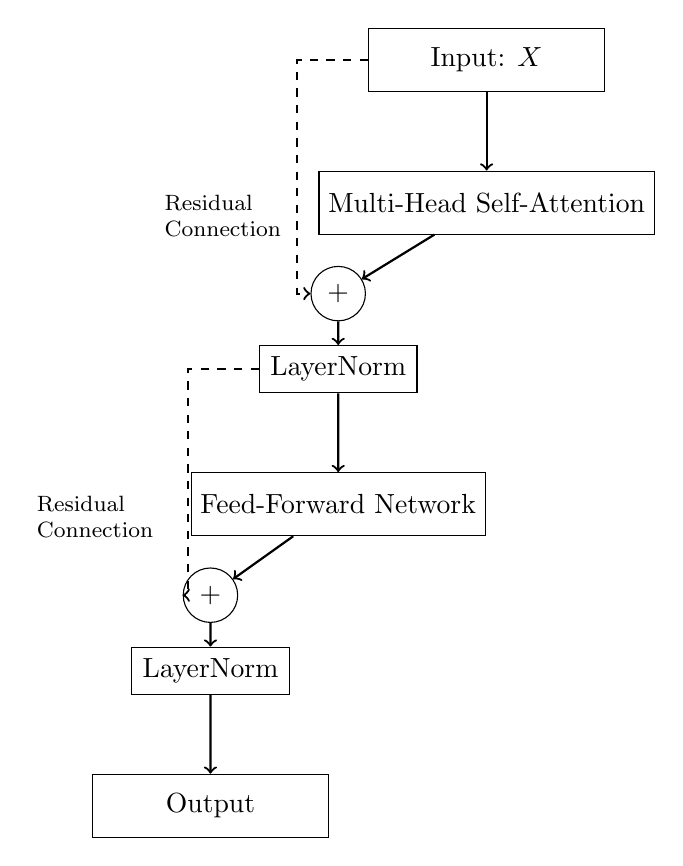
\begin{tikzpicture}[scale=0.9, node distance=1cm]
\node[draw, rectangle, minimum width=3cm, minimum height=0.8cm] (input) {Input: $X$};

\node[draw, rectangle, minimum width=3cm, minimum height=0.8cm, below=of input] (attn) {Multi-Head Self-Attention};
\node[draw, circle, minimum size=0.6cm, below left=0.5cm and -0.5cm of attn] (add1) {+};
\node[draw, rectangle, minimum width=2cm, minimum height=0.6cm, below=0.3cm of add1] (ln1) {LayerNorm};

\node[draw, rectangle, minimum width=3cm, minimum height=0.8cm, below=of ln1] (ffn) {Feed-Forward Network};
\node[draw, circle, minimum size=0.6cm, below left=0.5cm and -0.5cm of ffn] (add2) {+};
\node[draw, rectangle, minimum width=2cm, minimum height=0.6cm, below=0.3cm of add2] (ln2) {LayerNorm};

\node[draw, rectangle, minimum width=3cm, minimum height=0.8cm, below=of ln2] (output) {Output};

\draw[->, thick] (input) -- (attn);
\draw[->, thick] (attn) -- (add1);
\draw[->, thick, dashed] (input.west) -- ++(-1,0) |- (add1.west);
\draw[->, thick] (add1) -- (ln1);
\draw[->, thick] (ln1) -- (ffn);
\draw[->, thick] (ffn) -- (add2);
\draw[->, thick, dashed] (ln1.west) -- ++(-1,0) |- (add2.west);
\draw[->, thick] (add2) -- (ln2);
\draw[->, thick] (ln2) -- (output);

\node[align=left, font=\footnotesize, above left=0.5cm of add1] {Residual\\Connection};
\node[align=left, font=\footnotesize, above left=0.5cm of add2] {Residual\\Connection};
\end{tikzpicture}
\end{center}

\textbf{Residual connections} (the skip connections) are crucial:
\begin{itemize}
\item Help gradients flow during backpropagation
\item Allow the model to learn identity mappings when needed
\item Enable training of very deep networks (12--24+ layers)
\end{itemize}

\textbf{Layer normalization} stabilizes training:
\begin{itemize}
\item Normalizes activations across the feature dimension
\item Reduces internal covariate shift
\item Makes the model less sensitive to initialization
\end{itemize}




\subsection{Cross-Attention vs. Self-Attention in the Decoder}

The Transformer decoder has \textbf{two} types of attention:

\begin{enumerate}
\item \textbf{Masked Self-Attention}: Within the target sequence, with causal masking
\begin{itemize}
\item $Q, K, V$ all from previous decoder layer
\item Each position attends only to previous positions
\end{itemize}

\item \textbf{Cross-Attention}: From target to source (same as last lecture!)
\begin{itemize}
\item $Q$ from decoder (the query)
\item $K, V$ from encoder output (the memory bank)
\item No causal mask needed (entire source is available)
\end{itemize}
\end{enumerate}

\section{Interpretation: Memory, Retrieval, and the Roles of Attention and FFN}

We often hear that Large Language Models (LLMs) have ``memorized the internet." But how can a fixed-size model store terabytes of text? It cannot store it verbatim. It performs \textbf{lossy compression}. The true brilliance lies in \emph{how} it compresses and, crucially, \emph{how} it accesses that compressed knowledge. The Transformer architecture implements a crucial separation of concerns between its two main components: Attention and Feed-Forward Networks (FFNs).

\subsection{Intuition: The Efficient Librarian Analogy}

We can understand this separation through the analogy of an extraordinarily efficient librarian managing a library containing the entire internet.

\paragraph{Phase 1: Organizing the Library (Training).}
When the Transformer is trained, the librarian reads, summarizes (lossy compression), and organizes the collection.
\begin{itemize}
   \item \textbf{Efficient Shelving (The Embedding Space):} The librarian organizes summaries by placing \emph{similar concepts next to each other} (e.g., ``Paris" near ``France"). This organizational system is the model's high-dimensional \textbf{vector space}, learned via gradient descent.
   \item \textbf{The Knowledge Store (FFNs as Memory):} The FFN layers act as the primary memory banks—the specialized bookshelves where the compressed knowledge is stored.
\end{itemize}

\paragraph{Phase 2: Answering a Request (Inference).}
When you provide a prompt (the \textbf{Query}), you are asking the librarian a question.
\begin{enumerate}
   \item \textbf{The Efficient Search (Attention Mechanism):} The librarian instantly identifies the relevant sections because the library is organized by similarity. This is the \textbf{Attention Mechanism} ($QK^T$ operation). It compares the Query (request) against the Keys (index) to find relevant concepts. Attention decides \emph{where} to look.
   \item \textbf{Retrieval and Application (The FFN's Role):} Once attention has gathered the relevant context, the FFN layers (the bookshelves) are accessed to retrieve the specific knowledge (\textbf{Values}) associated with the context to determine the next word. The FFN decides \emph{what} information to apply.
\end{enumerate}

\begin{tcolorbox}[colback=blue!5!white, colframe=blue!75!black, title=Separation of Concerns]
The architecture implements a clear division of labor:
\begin{itemize}
   \item \textbf{Attention} performs \textbf{content-based routing/mixing} across tokens (the librarian finding the right aisles).
   \item \textbf{FFNs} perform \textbf{token-local computation} and act as the dense, associative memory (the content on the shelves).
\end{itemize}
\end{tcolorbox}

\subsection{The Mechanism: FFNs as Associative Memory}

We previously interpreted the FFN as a nonlinear feature map $\phi(z)$ required for the attention mechanism to function like a learned kernel. Complementary to this, the FFN acts as a \textbf{high-capacity associative memory} that turns local context features (gathered by attention) into next-token evidence.

Concretely, for a token representation $z\in\mathbb{R}^{d_{\mathrm{model}}}$, a 2-layer FFN (ReLU/GELU) with residual is:
\[
\underbrace{z'}_{\text{to next sublayer}}
= z + W_2\,\sigma(W_1\,\mathrm{LN}(z)+b_1)+b_2.
\]

\paragraph{Key–Value (KV) View of a Dense FFN.}
We can understand how the FFN stores knowledge by looking at its structure componentwise (using ReLU activation, $[\cdot]_+=\max(\cdot,0)$, for clarity):
\[
\mathrm{FFN}(z) \;=\; \sum_{j=1}^{m} \underbrace{\big[\,w_{1j}^{\top} z + b_{1j}\,\big]_+}_{\text{gate } g_j(z)}
\;\underbrace{v_j}_{\text{value}},\qquad
v_j := \text{$j$th column of }W_2,
\]
where $w_{1j}^{\top}$ is the $j$th row of $W_1$. Each hidden unit defines:
\begin{itemize}[leftmargin=1.2em]
\item a \emph{key} (or selector) $w_{1j}$ that decides when the neuron fires ($g_j(z)>0$). This corresponds to the first layer ($W_1$) recognizing specific patterns or contexts.
\item a \emph{value} vector $v_j$ that is \emph{written} to the token stream when that key matches. This corresponds to the second layer ($W_2$) providing the associated knowledge.
\end{itemize}
Thus, a dense FFN is a large bank of KV pairs $\{(w_{1j},v_j)\}_{j=1}^m$ softly selected by the input context $z$. (This structure is sometimes referred to as a dense Mixture-of-Experts, MoE).

\paragraph{Why this is ``Memorization''.}
Training pushes $w_{1j}$ (the key) to activate on specific contextual patterns (e.g., the representation elicited by “\texttt{The Shawshank}”), and $v_j$ (the value) to point toward directions that raise the correct next-token logits (e.g., “\texttt{Redemption}”). The pair \((w_{1j},v_j)\) thereby \emph{stores} the association $\mathcal{C}\mapsto \texttt{Redemption}$. Many such pairs superpose, yielding a sparse, distributed memory.

\paragraph{Why this is also ``Interpolation''.}
Because the gate $g_j(z)$ varies smoothly with $z$ (ReLU/GELU are Lipschitz), nearby contexts activate similar neuron subsets with similar strengths. The FFN therefore implements a \emph{piecewise-linear kernel smoother}:
\[
\mathrm{FFN}(z)\;=\;\sum_j g_j(z)\,v_j
\quad\Longleftrightarrow\quad
\text{``average'' values of neurons whose keys match $z$.}
\]
This is the tokenwise analogue of our kernel-regression story. It allows the model to generalize: even if it hasn't seen the exact context $z$ before, it can interpolate between known facts.

\subsection{Cooperation between Attention and FFN}

The Transformer architecture relies on the interplay between these two components:

\begin{enumerate}[leftmargin=1.2em]
\item \textbf{Attention = Retrieval/Routing.} MHA aggregates information from other positions across the sequence to form the context $z$.
\item \textbf{FFN = Compute/Memory.} Given $z$, the FFN fires a sparse set of KV “experts” to convert that routed context into concrete logit pushes for the next token.
\item \textbf{Residual Stacking.} Alternating \(\text{MHA}\) and \(\text{FFN}\) layers yields: \(\underbrace{\text{route}}_{\text{MHA}}\rightarrow\underbrace{\text{compute/memorize}}_{\text{FFN}}\rightarrow\cdots\), enabling long-range composition (via routing) and local rule/fact application (via memory).
\end{enumerate}

The concrete parameters that encode phrase/fact associations reside largely in the FFN. This is practical because FFN layers (typically width $\approx 4d_{\mathrm{model}}$) dominate the parameter count, providing far more storage capacity (parameter mass) than the comparatively small $Q,K,V$ projections in the attention layers.

\[
\boxed{\text{Attention decides \emph{where} to look; FFN decides \emph{what} to write/add for prediction.}}
\]


\section{Implementation: Self-Attention Layer}

\begin{lstlisting}[language=Python, caption=Self-Attention Implementation]
import torch
import torch.nn as nn
import math

class SelfAttention(nn.Module):
   def __init__(self, d_model, d_k, d_v, dropout=0.1):
     super().__init__()
     self.d_k = d_k
     
     # Linear projections for Q, K, V
     self.W_q = nn.Linear(d_model, d_k, bias=False)
     self.W_k = nn.Linear(d_model, d_k, bias=False)
     self.W_v = nn.Linear(d_model, d_v, bias=False)
     
     self.dropout = nn.Dropout(dropout)
     
   def forward(self, x, mask=None):
     ``""
     x: (batch, seq_len, d_model)
     mask: (batch, seq_len, seq_len) or (seq_len, seq_len)
         True for positions to keep, False for masked positions
     ``""
     # Project to Q, K, V
     Q = self.W_q(x)  # (batch, seq_len, d_k)
     K = self.W_k(x)  # (batch, seq_len, d_k)
     V = self.W_v(x)  # (batch, seq_len, d_v)
     
     # Compute attention scores
     scores = torch.matmul(Q, K.transpose(-2, -1)) / math.sqrt(self.d_k)
     # scores shape: (batch, seq_len, seq_len)
     
     # Apply mask if provided
     if mask is not None:
       scores = scores.masked_fill(mask == 0, float('-inf'))
     
     # Softmax to get attention weights
     attention_weights = torch.softmax(scores, dim=-1)
     attention_weights = self.dropout(attention_weights)
     
     # Weighted sum of values
     output = torch.matmul(attention_weights, V)
     # output shape: (batch, seq_len, d_v)
     
     return output, attention_weights
\end{lstlisting}

\section{Multi-Head Self-Attention}
A single attention head computes its output as a weighted average of the value vectors across all positions. This averaging mechanism can dilute information and inhibit the model's ability to focus sharply on multiple aspects of the sequence simultaneously.

Consider the diverse relationships in language: syntactic dependencies, semantic roles, coreference, and positional context. A single head must compress all these relationships into one weighted sum.

\begin{tcolorbox}[colback=gray!10!white, colframe=gray!50!black, title=The Resolution Trade-off]
As noted in Vaswani et al. (2017), achieving a constant number of operations comes ``at the cost of reduced effective resolution due to averaging attention-weighted positions.''
\end{tcolorbox}

\subsection{The Multi-Head Solution}

We counteract this reduction in resolution using \textbf{Multi-Head Attention (MHA)}. MHA is the mechanism that allows the model to capture the complexity and nuance of language without sacrificing the efficiency of the attention mechanism.

\begin{tcolorbox}[colback=blue!5!white, colframe=blue!75!black, title={Different Subspaces, Joint Attention}]
``Multi-head attention allows the model to jointly attend to information from different representation subspaces at different positions. With a single attention head, averaging inhibits this.'' (Vaswani et al., 2017)
\end{tcolorbox}

Instead of performing a single attention function with $d_{model}$-dimensional keys, values, and queries, we linearly project the inputs into $h$ different subspaces, each with a smaller dimension (typically $d_k = d_{model}/h$). We then perform the attention function in parallel on each subspace.

\begin{equation}
\text{head}_i = \text{Attention}(QW_Q^i, KW_K^i, VW_V^i)
\end{equation}

\begin{itemize}
   \item \textbf{Representation Subspaces:} Each head operates within its own learned subspace ($W_Q^i, W_K^i, W_V^i$). This allows different heads to specialize in different types of relationships (e.g., one head for syntax, another for local context).
   \item \textbf{Concatenation:} The outputs of all heads are concatenated and passed through a final linear projection ($W_O$), preserving the distinct information gathered by each.
\end{itemize}

\begin{equation}
\text{MultiHead}(Q, K, V) = \text{Concat}(\text{head}_1, \ldots, \text{head}_h)W_O
\end{equation}

\subsection{Implementation}

In practice, we do not use $h$ separate sets of matrices. For computational efficiency, the projections for all heads are combined into single, large matrices ($W_Q, W_K, W_V$), and the dimensions are reshaped to calculate the heads in parallel.

\begin{lstlisting}[language=Python, caption=Multi-Head Self-Attention]
class MultiHeadSelfAttention(nn.Module):
   def __init__(self, d_model, num_heads, dropout=0.1):
     super().__init__()
     assert d_model % num_heads == 0
     
     self.d_model = d_model
     self.num_heads = num_heads
     self.d_k = d_model // num_heads
     
     # Single projections for all heads (more efficient)
     self.W_q = nn.Linear(d_model, d_model, bias=False)
     self.W_k = nn.Linear(d_model, d_model, bias=False)
     self.W_v = nn.Linear(d_model, d_model, bias=False)
     self.W_o = nn.Linear(d_model, d_model, bias=False)
     
     self.dropout = nn.Dropout(dropout)
     
   def forward(self, x, mask=None):
     """
     x: (batch, seq_len, d_model)
     """
     batch_size, seq_len, _ = x.shape
     
     # Linear projections and split into heads
     # (batch, seq_len, d_model) -> (batch, seq_len, num_heads, d_k)
     Q = self.W_q(x).view(batch_size, seq_len, self.num_heads, self.d_k)
     K = self.W_k(x).view(batch_size, seq_len, self.num_heads, self.d_k)
     V = self.W_v(x).view(batch_size, seq_len, self.num_heads, self.d_k)
     
     # Transpose to (batch, num_heads, seq_len, d_k)
     # This allows for efficient parallel computation across heads
     Q = Q.transpose(1, 2)
     K = K.transpose(1, 2)
     V = V.transpose(1, 2)
     
     # Compute scaled dot-product attention
     # (b, h, T, d_k) @ (b, h, d_k, T) -> (b, h, T, T)
     scores = torch.matmul(Q, K.transpose(-2, -1)) / math.sqrt(self.d_k)
     
     if mask is not None:
       # Expand mask for all heads
       mask = mask.unsqueeze(1)  # (batch, 1, seq_len, seq_len)
       scores = scores.masked_fill(mask == 0, float('-inf'))
     
     attention_weights = torch.softmax(scores, dim=-1)
     attention_weights = self.dropout(attention_weights)
     
     # (b, h, T, T) @ (b, h, T, d_k) -> (b, h, T, d_k)
     attn_output = torch.matmul(attention_weights, V)
     
     # Concatenate heads
     # (b, h, T, d_k) -> (b, T, h, d_k) -> (b, T, d_model)
     attn_output = attn_output.transpose(1, 2).contiguous()
     attn_output = attn_output.view(batch_size, seq_len, self.d_model)
     
     # Final linear projection (W_O)
     output = self.W_o(attn_output)
     
     return output, attention_weights
\end{lstlisting}
\section{Positional Encoding Implementation}

\begin{lstlisting}[language=Python, caption=Sinusoidal Positional Encoding]
class PositionalEncoding(nn.Module):
   def __init__(self, d_model, max_len=5000, dropout=0.1):
     super().__init__()
     self.dropout = nn.Dropout(dropout)
     
     # Create positional encoding matrix
     pe = torch.zeros(max_len, d_model)
     position = torch.arange(0, max_len).unsqueeze(1).float()
     
     # Compute the div term: 1 / (10000^(2i/d_model))
     div_term = torch.exp(
       torch.arange(0, d_model, 2).float() * 
       -(math.log(10000.0) / d_model)
     )
     
     # Apply sin to even indices, cos to odd indices
     pe[:, 0::2] = torch.sin(position * div_term)
     pe[:, 1::2] = torch.cos(position * div_term)
     
     # Add batch dimension
     pe = pe.unsqueeze(0)  # (1, max_len, d_model)
     
     # Register as buffer (not a parameter, but part of state)
     self.register_buffer('pe', pe)
     
   def forward(self, x):
     ``""
     x: (batch, seq_len, d_model)
     ``""
     # Add positional encoding to input
     # pe is (1, max_len, d_model), we take first seq_len positions
     x = x + self.pe[:, :x.size(1), :]
     return self.dropout(x)
\end{lstlisting}

\section{Why Transformers Are Revolutionary}

\subsection{Training Efficiency}

\begin{tcolorbox}[colback=green!5!white, colframe=green!50!black, title=Parallel Training]
Every position in every layer can be computed \textbf{simultaneously}.

For a sequence of length 512 with batch size 32:
\begin{itemize}
\item \textbf{RNN}: 512 sequential steps per example = 512 sequential operations minimum
\item \textbf{Transformer}: All 512 positions computed in parallel = constant time per layer
\end{itemize}

On modern GPUs with thousands of cores, this means:
\begin{itemize}
\item Training is 10--100$\times$ faster
\item We can train on much larger datasets
\item We can use much larger models
\end{itemize}
\end{tcolorbox}

\subsection{Scaling Properties}

The Transformer's architecture enables unprecedented scaling:

\begin{enumerate}
\item \textbf{Scalable to billions of parameters}: Parallel computation allows training massive models (GPT-3: 175B parameters, GPT-4: estimated 1.7T parameters)

\item \textbf{Better with more data}: Unlike RNNs which saturate, Transformers continue improving with more data

\item \textbf{Transfer learning}: Pre-train once on massive data, fine-tune for specific tasks

\item \textbf{Hardware-friendly}: Modern accelerators (GPUs/TPUs) are optimized for the matrix operations in self-attention
\end{enumerate}

\subsection{Capturing Complex Patterns}

Direct connections between all positions enable:
\begin{itemize}
\item \textbf{Long-range dependencies}: Word 1 can directly influence word 500 in a single layer
\item \textbf{Syntax modeling}: Capturing grammatical relationships across the sentence
\item \textbf{Semantic relationships}: Understanding thematic connections
\item \textbf{Multiple perspectives}: Different heads learn different types of relationships
\end{itemize}

\section{Limitations and Open Questions}

\subsection{The Quadratic Bottleneck}

Self-attention has $O(n^2)$ complexity with respect to sequence length:

\begin{itemize}
\item For sequences of 512 tokens: 262,144 attention computations
\item For sequences of 4,096 tokens: 16,777,216 attention computations (64$\times$ more!)
\item Memory scales quadratically too: storing the $n \times n$ attention matrix
\end{itemize}

This limits Transformers to relatively short contexts ($\sim$2000--8000 tokens in practice).

\textbf{Active research area}:
\begin{itemize}
\item Sparse attention patterns (only attend to a subset of positions)
\item Linear attention approximations (kernel methods)
\item Hierarchical approaches (attend at multiple granularities)
\item Memory-efficient implementations (FlashAttention, don't materialize the full attention matrix)
\end{itemize}

\subsection{Interpretability Challenges}

While attention weights are often visualized, interpreting what the model ``learned'' is difficult:
\begin{itemize}
\item Multiple layers with multiple heads create complex interaction patterns
\item Attention weights don't necessarily correspond to importance
\item Residual connections mix information from many layers
\end{itemize}

\subsection{Training Stability}

Transformers can be unstable to train:
\begin{itemize}
\item Careful initialization is crucial
\item Learning rate warmup is essential (start small, gradually increase)
\item Layer normalization placement matters (pre-norm vs. post-norm)
\item Very deep models can suffer from gradient issues
\end{itemize}

\section{Summary: The Transformation is Complete}

\subsection{From RNNs to Transformers}

\begin{center}
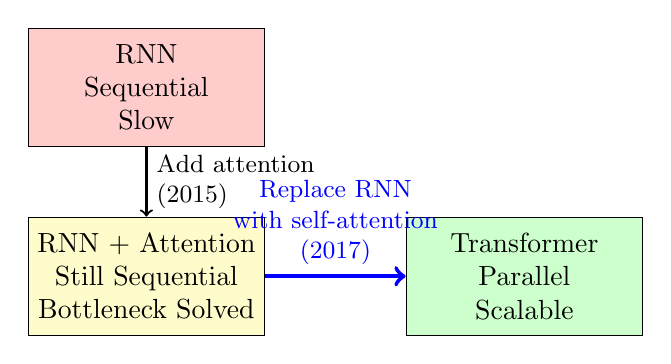
\begin{tikzpicture}[scale=0.8]
\node[draw, rectangle, minimum width=3cm, minimum height=1.5cm, fill=red!20, align=center] (rnn) at (0,3) {RNN\\Sequential\\Slow};

\node[draw, rectangle, minimum width=3cm, minimum height=1.5cm, fill=yellow!20, align=center] (rnn_attn) at (0,0) {RNN + Attention\\Still Sequential\\Bottleneck Solved};

\node[draw, rectangle, minimum width=3cm, minimum height=1.5cm, fill=green!20, align=center] (transformer) at (6,0) {Transformer\\Parallel\\Scalable};

\draw[->, thick] (rnn) -- (rnn_attn) node[midway, right, font=\small, align=left] {Add attention\\(2015)};
\draw[->, ultra thick, blue] (rnn_attn) -- (transformer) node[midway, above, font=\small, align=center] {Replace RNN\\with self-attention\\(2017)};
\end{tikzpicture}
\end{center}

\subsection{Key Takeaways}

\begin{enumerate}
\item \textbf{Self-attention} is attention where Q, K, V all come from the same sequence
\begin{itemize}
\item Each position refines its representation by attending to related positions
\item Enables parallel computation (unlike RNNs)
\item Provides direct connections between all positions ($O(1)$ path length)
\end{itemize}

\item \textbf{Positional encoding} is essential because self-attention has no notion of order
\begin{itemize}
\item Sine/cosine functions provide learnable relative position information
\item Bounded, deterministic, and generalizable to unseen lengths
\end{itemize}

\item \textbf{The Transformer} replaces recurrence with stacked self-attention layers
\begin{itemize}
\item Encoder: self-attention + feed-forward networks
\item Decoder: masked self-attention + cross-attention + feed-forward networks
\item Residual connections and layer normalization enable deep networks
\end{itemize}

\item \textbf{Causal masking} in the decoder prevents ``cheating''
\begin{itemize}
\item Position $t$ can only attend to positions $\leq t$
\item Preserves autoregressive property
\end{itemize}

\item \textbf{Feed-forward networks} provide the necessary non-linearity
\begin{itemize}
\item Self-attention alone is linear (+ normalization)
\item FFN enables complex feature transformations
\item Applied independently to each position
\end{itemize}

\item \textbf{Transformers scale} in ways RNNs cannot
\begin{itemize}
\item Parallel training enables massive models
\item Billions of parameters are practical
\item Continue improving with more data
\end{itemize}
\end{enumerate}

\subsection{The Big Picture}

\begin{tcolorbox}[colback=blue!5!white, colframe=blue!75!black, title=The Attention Revolution]
The key insight: \textbf{Attention is not just useful---it's sufficient}.

We don't need recurrence. We don't need convolution. Self-attention plus positional encoding plus non-linear transformations are \textbf{all you need} to build powerful sequence models.

This insight has transformed not just NLP, but computer vision (Vision Transformers), speech, reinforcement learning, and more.

The Transformer architecture is the foundation of:
\begin{itemize}
\item GPT (generative pre-trained transformers)
\item BERT (bidirectional encoder representations)
\item T5 (text-to-text transfer transformer)
\item Vision Transformers (ViT)
\item Multimodal models (CLIP, Flamingo)
\item And virtually all state-of-the-art language models today
\end{itemize}
\end{tcolorbox}

\section{Looking Ahead}

\subsection{Next Steps in This Course}

We've now covered the fundamental architecture. Coming lectures will explore:

\begin{itemize}
\item \textbf{Training Transformers}: Optimization tricks, warmup schedules, mixed precision
\item \textbf{Pre-training and Transfer Learning}: How to leverage massive unlabeled data
\item \textbf{Scaling Laws}: Why bigger models + more data = better performance
\item \textbf{Efficient Transformers}: Techniques to handle longer sequences
\item \textbf{Vision Transformers}: Adapting Transformers to images
\item \textbf{Multimodal Learning}: Unified architectures for text, images, and more
\end{itemize}

\subsection{Research Frontiers}

Open questions driving current research:

\begin{enumerate}
\item How can we scale to much longer contexts (100K+ tokens)?
\item What are the fundamental limits of the scaling laws?
\item How can we make Transformers more interpretable?
\item What architectural improvements are possible?
\item How do we handle structured data and complex reasoning?
\end{enumerate}

\section{Exercises}

\begin{enumerate}
\item \textbf{Positional Encoding Analysis}:
\begin{itemize}
\item Implement the sinusoidal positional encoding
\item Visualize the encoding for the first 50 positions and 128 dimensions
\item Compute the cosine similarity between position encodings at offsets 1, 5, 10, and 20
\item What patterns do you observe?
\end{itemize}

\item \textbf{Self-Attention Patterns}:
\begin{itemize}
\item Implement a single-head self-attention layer from scratch
\item Create a simple sequence: ``The cat sat on the mat''
\item Visualize the attention weights matrix
\item Which words attend most strongly to each other? Why?
\end{itemize}

\item \textbf{Causal Masking}:
\begin{itemize}
\item Implement causal masking for decoder self-attention
\item Verify that position $t$ cannot attend to positions $> t$
\item Compare the attention patterns with and without masking
\end{itemize}

\item \textbf{Architecture Comparison}:
\begin{itemize}
\item Calculate the number of operations for RNN, CNN, and self-attention for a sequence of length 100, 1000, and 10000
\item Assume $d = 512$, kernel size $k = 3$ for CNN
\item Plot the complexity as a function of sequence length
\item At what sequence length does self-attention become more expensive than RNN?
\end{itemize}

\item \textbf{Multi-Head Attention Analysis}:
\begin{itemize}
\item Implement multi-head self-attention with 4 heads
\item Train on a simple task (e.g., copy task or sorting)
\item Visualize what each head learns
\item Are there redundant heads? What patterns do you see?
\end{itemize}

\item \textbf{Positional Encoding Ablation}:
\begin{itemize}
\item Train a small Transformer with and without positional encoding
\item Test on a task where position matters (e.g., ``reverse the sequence'')
\item What happens to performance? Why?
\end{itemize}

\item \textbf{Implementation Challenge}:
\begin{itemize}
\item Build a complete Transformer encoder from scratch
\item Stack 2--4 layers with multi-head attention and feed-forward networks
\item Include residual connections and layer normalization
\item Train on a simple sequence classification task
\end{itemize}

\item \textbf{Attention Pattern Analysis}:
Use a pre-trained model (e.g., from HuggingFace) and:
\begin{itemize}
\item Extract attention weights for a sample sentence
\item Identify heads that focus on syntactic relationships (e.g., subject-verb)
\item Identify heads that focus on semantic relationships
\item Are there heads that seem to focus on positional patterns?
\end{itemize}

\item \textbf{Complexity Deep Dive}:
\begin{itemize}
\item Derive the $O(n^2 d)$ complexity for self-attention
\item Derive the $O(nd^2)$ complexity for RNNs
\item For what values of $n$ and $d$ is self-attention more efficient (in FLOPs)?
\item Consider parallelization: how does this change the comparison?
\end{itemize}

\item \textbf{Design Challenge}:
Propose a modification to self-attention that:
\begin{itemize}
\item Reduces the $O(n^2)$ complexity
\item Maintains the ability to capture long-range dependencies
\item Is still parallelizable
\item Justify your design choices and discuss trade-offs
\end{itemize}
\end{enumerate}

\section{Further Reading}

\subsection{Foundational Papers}

\begin{itemize}
\item Vaswani, A., et al. (2017). \textbf{Attention Is All You Need}. NeurIPS. \textit{The original Transformer paper---essential reading.}

\item Devlin, J., et al. (2019). \textbf{BERT: Pre-training of Deep Bidirectional Transformers for Language Understanding}. NAACL.

\item Radford, A., et al. (2019). \textbf{Language Models are Unsupervised Multitask Learners}. (GPT-2)

\item Dosovitskiy, A., et al. (2021). \textbf{An Image is Worth 16x16 Words: Transformers for Image Recognition at Scale}. ICLR. \textit{Vision Transformers.}
\end{itemize}

\subsection{Efficient Transformers}

\begin{itemize}
\item Tay, Y., et al. (2020). \textbf{Efficient Transformers: A Survey}. \textit{Comprehensive overview of methods to reduce complexity.}

\item Kitaev, N., et al. (2020). \textbf{Reformer: The Efficient Transformer}. ICLR.

\item Dao, T., et al. (2022). \textbf{FlashAttention: Fast and Memory-Efficient Exact Attention with IO-Awareness}. NeurIPS.
\end{itemize}

\subsection{Analysis and Understanding}

\begin{itemize}
\item Clark, K., et al. (2019). \textbf{What Does BERT Look At? An Analysis of BERT's Attention}. ACL Workshop.

\item Rogers, A., et al. (2020). \textbf{A Primer on Neural Network Architectures for Natural Language Processing}. \textit{Excellent overview.}
\end{itemize}

\subsection{Textbooks}

\begin{itemize}
\item Zhang, A., et al. (2023). \textbf{Dive into Deep Learning}. Chapter 11: Attention Mechanisms and Transformers.

\item Jurafsky, D., \& Martin, J. H. (2023). \textbf{Speech and Language Processing} (3rd ed.). Chapter 10: Transformers and Large Language Models.
\end{itemize}


\section*{FFN as the Locus of Memorization \& Interpolation, and its Role Next to Attention}

\paragraph{Separation of concerns.}
In an attention block, \emph{attention} performs \textbf{content-based routing/mixing} across tokens, while the \emph{positionwise FFN} performs \textbf{token-local computation}. Concretely, for a token representation $z\in\mathbb{R}^{d_{\mathrm{model}}}$, a 2-layer FFN (ReLU/GELU) with residual is
\[
\underbrace{z'}_{\text{to next sublayer}}
= z + W_2\,\sigma(W_1\,\mathrm{LN}(z)+b_1)+b_2.
\]
Previously we interpret this as a nonlinear feature map $\phi(z)=\mathrm{LN}\!\big(z+ \mathrm{FFN}(\mathrm{LN}(z))\big)$ on which scaled dot-product attention applies an (efficient) bilinear similarity. Also FFN contributes the most memorization and interpolation: \textbf{the FFN is a high-capacity associative memory that turns local context features into next-token evidence.}

\paragraph{Key–value (KV) view of a dense FFN.}
Write the FFN (with ReLU for clarity) componentwise:
\[
\mathrm{FFN}(z) \;=\; \sum_{j=1}^{m} \underbrace{\big[\,w_{1j}^{\top} z + b_{1j}\,\big]_+}_{\text{gate } g_j(z)}
\;\underbrace{v_j}_{\text{value}},\qquad
v_j := \text{$j$th column of }W_2,
\]
where $w_{1j}^{\top}$ is the $j$th row of $W_1$ and $[\cdot]_+=\max(\cdot,0)$. Each hidden unit defines:
\begin{itemize}[leftmargin=1.2em]
\item a \emph{key} (or selector) $w_{1j}$ that decides when the neuron fires (\(g_j(z)>0\) iff $z$ lies on one side of a hyperplane),
\item a \emph{value} vector $v_j$ that is \emph{written} to the token stream when that key matches.
\end{itemize}
Thus a dense FFN is a \emph{dense MoE}: a large bank of KV pairs $\{(w_{1j},v_j)\}_{j=1}^m$ softly selected by $z$. Training pushes $w_{1j}$ to activate on specific contextual patterns (e.g., the phrase embedding of “\texttt{The Shawshank}”), and $v_j$ to point toward representation directions that raise the right next-token logits (e.g., “\texttt{Redemption}”).

\paragraph{Why this is ``memorization''.}
Let $E\in\mathbb{R}^{|\mathcal{V}|\times d_{\mathrm{model}}}$ be the LM head (tied or untied). The logit of token $v$ after an FFN+\emph{residual} is
\[
\ell_v \;=\; \langle E_v,\, z \rangle \;+\; \sum_{j:\,g_j(z)>0}\; g_j(z)\;\langle E_v,\, v_j\rangle.
\]
A neuron $j$ whose value $v_j$ aligns with $E_v$ contributes a positive bump to $\ell_v$ whenever its gate $g_j(z)$ is on. During training on many occurrences of a context $\mathcal{C}$ (e.g., the representation elicited by “The Shawshank”), gradients \emph{co-adapt} $w_{1j}$ to fire on $\mathcal{C}$ and $v_j$ to align with $E_{\texttt{Redemption}}$. The pair \((w_{1j},v_j)\) thereby \emph{stores} the association $\mathcal{C}\mapsto \texttt{Redemption}$. Many such pairs superpose, yielding a sparse, distributed memory.

\paragraph{Why this is also ``interpolation''.}
Because $g_j(z)$ varies smoothly with $z$ (ReLU/GELU are Lipschitz), nearby contexts activate similar neuron subsets with similar strengths. The FFN therefore implements a \emph{piecewise-linear kernel smoother}:
\[
\mathrm{FFN}(z)\;=\;\sum_j g_j(z)\,v_j
\quad\Longleftrightarrow\quad
\text{``average'' values of neurons whose keys match $z$.}
\]
This is the tokenwise analogue of our kernel-regression story: the FFN supplies the nonlinear lift $\phi(z)$ and performs a local interpolation from context to next-token evidence, while \emph{attention} provides the cross-token retrieval that builds $z$ in the first place.

\paragraph{How attention and FFN cooperate.}
\begin{enumerate}[leftmargin=1.2em]
\item \textbf{Attention = retrieval/routing.} MHA aggregates information from other positions to form $z$ (your $Q\!K^\top$ / kernel view).
\item \textbf{FFN = compute/memory.} Given $z$, the FFN fires a sparse set of KV “experts” to convert that routed context into concrete logit pushes. Capacity and facts mostly live in $W_1,W_2$ (they dominate parameters).
\item \textbf{Residual stacking.} Alternating \(\text{MHA}\) and \(\text{FFN}\) layers yields: \(\underbrace{\text{route}}_{\text{MHA}}\rightarrow\underbrace{\text{compute/memorize}}_{\text{FFN}}\rightarrow\cdots\), enabling long-range composition (via routing) and local rule/fact application (via memory).
\end{enumerate}


Our previous lecture’s kernel view says: \emph{FFN builds the nonlinear feature map} \(\phi(\cdot)\); attention performs efficient bilinear similarity and mixing on those features. Moreover \emph{the concrete parameters that encode phrase/fact associations and turn context into next-token logits reside largely in the FFN}, which acts as a content-addressed KV store and a smooth interpolator. Both are true and complementary:
\[
\boxed{\text{Attention decides \emph{where} to look; FFN decides \emph{what} to write/add for prediction.}}
\]

\paragraph{Why ``mostly FFN'' in practice.}
(i) Parameter mass: FFN layers (width $\approx 4d_{\mathrm{model}}$ or GLU variants) dominate parameter count, so they can store far more associations than the comparatively small $Q,K,V$ projections. (ii) Locality: tokenwise residual updates directly shape the LM head’s logits. (iii) Smoothness: gated sums yield stable piecewise-linear interpolation across similar contexts, “memorization \emph{and} interpolation” language.

\section{Interpretation: The Transformer as an Efficient Librarian of the Internet}

We often hear that Large Language Models (LLMs) have ``memorized the internet." But how can a fixed-size model store terabytes of text? The answer is that it cannot store it verbatim. It performs \textbf{lossy compression}. The true brilliance lies in \emph{how} it compresses and, crucially, \emph{how} it accesses that compressed knowledge.

We can understand this through the analogy of an extraordinarily efficient librarian managing a library containing the entire internet.

\subsection{Phase 1: Organizing the Library (Training and Compression)}

When the Transformer is trained, it is akin to the librarian reading, summarizing, and organizing the vast collection.

\begin{itemize}
   \item \textbf{Lossy Compression (Summarization):} The librarian cannot remember every word of every book. Instead, they extract key concepts, facts, relationships, and linguistic patterns. These summaries are stored, not the raw text.
   \item \textbf{Efficient Shelving (The Embedding Space):} The librarian organizes these summaries using a sophisticated system. Crucially, \emph{similar concepts are placed next to each other}. ``Paris" is placed near ``France" and ``Eiffel Tower." This organizational system is the model's high-dimensional \textbf{vector space}. A ``shelf" is not a physical location, but a region in this space, and the organization is learned via gradient descent.
   \item \textbf{The Knowledge Store (FFNs as Memory):} Where is the summarized knowledge actually stored? As we will explore in the next section, the Feed-Forward Network (FFN) layers act as the primary memory banks.
   \begin{tcolorbox}[colback=gray!10!white, colframe=gray!50!black, title=FFNs as the Bookshelves]
   We can view the FFNs as the specialized bookshelves or the detailed indexes of the library. They function as a massive, distributed key-value store:
   \begin{itemize}
     \item The first layer ($W_1$) learns \textbf{Keys} (the index lookup): recognizing specific contexts or patterns.
     \item The second layer ($W_2$) learns \textbf{Values} (the information): the knowledge associated with that pattern.
   \end{itemize}
   \end{tcolorbox}
\end{itemize}

The parameters of the model collectively define the structure of this library and the content of the summaries.

\subsection{Phase 2: Answering a Request (Inference and Retrieval)}

When you provide a prompt, you are a patron asking the librarian a question.

\begin{enumerate}
   \item \textbf{The Query:} The prompt is transformed into a vector representation—the \textbf{Query}. This represents the patron's information need.
   \item \textbf{The Efficient Search (Attention Mechanism):} The librarian doesn't check every summary on every shelf. Because the library is organized by similarity, the librarian can instantly identify the relevant sections.
   \begin{itemize}
     \item This is the core of the \textbf{Attention Mechanism} (the $QK^T$ operation). It compares the Query (the request) against the Keys (the organizational index) to find the most relevant internalized concepts.
     \item This aligns perfectly with the \textbf{Kernel Regression} view we discussed: the model computes a similarity score (the learned kernel) between the prompt and the stored data, focusing on the most similar items. Attention decides \emph{where} to look.
   \end{itemize}
   \item \textbf{Retrieval and Synthesis:} The librarian retrieves the relevant summaries (the \textbf{Values}) from those sections. Crucially, they synthesize them into a coherent answer. This is the weighted sum of the Values, guided by the attention scores.
   \item \textbf{Applying Knowledge (The FFN's Role):} Once attention has gathered the relevant context, the FFN layers process this information. The FFNs access the specific knowledge associated with the context to determine the next word. The FFN decides \emph{what} information to retrieve and apply.
\end{enumerate}

\begin{tcolorbox}[colback=blue!5!white, colframe=blue!75!black, title=The Power of Organization and Separation of Concerns]
This analogy highlights why Transformers are so efficient. The massive parallelism of the architecture allows the ``librarian" to check millions of ``summaries" simultaneously, and the learned organization ensures this search is incredibly fast.

The architecture implements a crucial separation of concerns:
\begin{itemize}
   \item \textbf{Attention} acts as the dynamic search and routing mechanism (the librarian finding the right aisles).
   \item \textbf{FFNs} act as the dense, associative memory storing the compressed knowledge of the internet (the content on the shelves).
\end{itemize}
\end{tcolorbox}

\end{document}